\documentclass[journal]{IEEEtran}

% ---- packages ----
\usepackage[T1]{fontenc}
\usepackage[utf8]{inputenc}
\usepackage{amsmath,amssymb,amsfonts}
\usepackage{graphicx}
\usepackage{booktabs}
\usepackage{array}
\usepackage{url}
\usepackage{xcolor}
\usepackage[hidelinks]{hyperref}
\usepackage{orcidlink}
\usepackage{balance}

\graphicspath{{../figures/}}

% keep floats near their reference
\renewcommand{\topfraction}{0.92}
\renewcommand{\bottomfraction}{0.75}
\renewcommand{\textfraction}{0.08}
\renewcommand{\floatpagefraction}{0.80}

\newcommand{\dsname}[1]{\textit{#1}}

\begin{document}

\title{Atalaya: A Calibrated Multi-Evidence Affinity Graph\\ over an Open-Data Catalog,\\ with an Empirical False-Discovery Gate}

\author{Felipe~Santiba\~nez-Leal~\orcidlink{0000-0002-0150-3246}%
\thanks{F. Santiba\~nez-Leal is with the CAOS open-research programme, Santiago, Chile
(e-mail: fsantibanez@gmail.com; ORCID 0000-0002-0150-3246).}%
\thanks{Preprint, 2026. Source, committed artifacts, and a live instance are open (MIT):
\url{https://github.com/fsantibanezleal/CAOS_ATALAYA}; \url{https://atalaya.fasl-work.com}.}}

\markboth{Preprint, 2026}%
{Santiba\~nez-Leal: A Calibrated Multi-Evidence Affinity Graph over an Open-Data Catalog}

\maketitle

\begin{abstract}
Open-data portals publish thousands of datasets as a flat searchable list, but the relational knowledge that
makes the data useful, which datasets can be joined, which describe the same thing, and which actually correlate
when aligned by a common key, stays implicit and is infeasible to recover by hand. Existing dataset-discovery
tools each rank relatedness on a \emph{single} signal (value containment for joinability, embedding cosine for
semantic search, statistical association for correlation mining), and each signal is individually misleading:
two datasets can be embedding-similar yet share no join key, joinable on \dsname{year} yet describe unrelated
phenomena, or correlate spuriously through a shared driver. We present Atalaya, a system that harvests a national
open-data catalog (1{,}017 datasets from Chile's Data Observatory; a 303-dataset, 24.8~GB government subset
mirrored and profiled in full), mines five orthogonal kinds of cross-dataset relation into an explorable
knowledge graph, and ranks pairwise relatedness with a novel \emph{calibrated multi-evidence affinity}. The
affinity fuses three orthogonal evidences into one interpretable $[0,1]$ score after passing each through its
\emph{empirical null distribution}, so the score means ``stronger than chance'' rather than ``large raw number'',
and it down-weights any evidence that contradicts the others. Two design choices make the graph trustworthy
rather than merely plausible. First, the correlation edges pass an \emph{empirical false-discovery gate}: on the
same alignments with the keys shuffled, $343$ candidate correlations yield $0$ survivors under a permutation null
with Benjamini--Hochberg control (empirical false-discovery rate $0.00$), so the $24$ correlations reported on
real data are believable. Second, the semantic encoder is measured honestly against a classical lexical
baseline, and we report the modest true margin ($+0.014$ top-$5$ neighbour-theme coherence over TF--IDF) rather
than overselling it. Every edge carries its evidence, the whole affinity is pure \texttt{numpy} so the browser
recomputes it live as an analyst reweights the evidences, and all figures are regenerated deterministically from
the committed artifacts. We give the method, the adversarial validation, and an explicit account of what the
graph does and does not license.
\end{abstract}

\begin{IEEEkeywords}
Dataset discovery, data integration, joinability, knowledge graph, semantic search, correlation mining,
false-discovery rate, null calibration, open data, reproducibility.
\end{IEEEkeywords}

\section{Introduction}

\IEEEPARstart{A}{national} open-data portal is a public good that undersells itself. Chile's Data Observatory,
like most portals built on the FAIR principles~\cite{fair}, exposes over a thousand datasets as a flat,
searchable list with per-dataset metadata. The list answers \emph{what} datasets exist. It does not answer the
question an analyst actually has, which is \emph{how they connect}: which two tables can be joined and on what
column, which describe the same phenomenon under different names, and which carry indicators that genuinely move
together when aligned by \dsname{comuna} (municipality) or region. That relational structure is the difference
between a thousand isolated files and a usable data fabric, and at the scale of a national catalog it cannot be
recovered by hand: the number of candidate dataset pairs is quadratic in the catalog size, and most pairs are
unrelated.

The database and information-retrieval communities have built strong tools for pieces of this problem. Data
discovery and augmentation systems such as Aurum~\cite{aurum} and Auctus~\cite{auctus} index a corpus and, given
a query table, return joinable or unionable tables; joinability at scale rests on estimating value-set
containment from compact sketches (MinHash~\cite{minhash}, sharpened by Lazo~\cite{lazo} and indexed by LSH
Ensemble~\cite{lshensemble}). Semantic catalog search embeds dataset text with a sentence
encoder~\cite{sbert,minilm} and ranks by cosine similarity; Google Dataset Search~\cite{gds} operationalises
this at web scale. Correlation miners look for statistical association between aligned indicator columns. Each of
these is excellent at its one signal, and each is, on its own, an unreliable notion of ``related''. A pair can be
embedding-similar because both datasets discuss ``population'' in prose, yet share no joinable key. A pair can be
perfectly joinable on \dsname{year} and describe entirely unrelated phenomena. A pair can correlate strongly and
spuriously because both track a common driver such as population or region~\cite{partialcorr}. Worse, a large
catalog is a multiple-testing minefield: mine thousands of candidate correlations without correction and a
handful will look significant by chance~\cite{bh}.

Atalaya's premise is that a trustworthy relatedness graph must do three things a single-signal ranker does not.
It must \textbf{fuse orthogonal evidences} so the strengths of one cover the blind spots of another. It must
\textbf{calibrate each evidence against a null model} so a score reflects surprise relative to random pairs, not
the raw magnitude of a signal whose scale is arbitrary. And it must be \textbf{honest and auditable}: every edge
should carry the evidence that justifies it, the statistical edges should survive an adversarial negative
control, and a learned component should be measured against a classical baseline with the real margin reported.
This paper contributes:

\begin{enumerate}
\item A \textbf{calibrated multi-evidence dataset-affinity score} (Section~\ref{sec:affinity}) that maps three
orthogonal raw evidences through their empirical null distributions and fuses them with reliability weights that
discount contradicting evidence. The score is in $[0,1]$, monotone, interpretable term-by-term, and cheap enough
(pure \texttt{numpy}) to recompute live in the browser under user reweighting.
\item An \textbf{honest relation-mining pipeline} (Section~\ref{sec:evidence}) that produces five orthogonal
edge kinds over a real national catalog, each recording its own evidence, with a correlation miner built from a
seeded permutation null, Benjamini--Hochberg false-discovery control, and a partial-correlation guard against
shared drivers.
\item An \textbf{adversarial validation} (Section~\ref{sec:validation}) centred on an \emph{empirical
false-discovery gate}: re-mining correlations on shuffled key alignments yields an empirical false-discovery
rate of $0.00$ ($0$ of $343$ candidate correlations survive), and the semantic encoder is benchmarked against a
TF--IDF lexical baseline with the modest true gain reported.
\item A \textbf{reproducible, explorable instance} over 1{,}017 datasets (Section~\ref{sec:results}), with all
derived artifacts committed and every figure in this paper regenerated deterministically from them.
\end{enumerate}

We are deliberate about scope (Section~\ref{sec:scope}): the graph reports where datasets \emph{can} be related
and how strongly relative to chance; it does not assert causation, and its tunables are set for one
government-Chile catalog. The value is not a claim of discovery but a method for turning a flat catalog into an
auditable relational map without inviting the reader to believe more than the evidence supports.

\section{Related Work}\label{sec:related}

\textbf{Dataset discovery and augmentation.} Aurum~\cite{aurum} builds an enterprise knowledge graph of columns
linked by content similarity and primary-key/foreign-key relationships; Auctus~\cite{auctus} is a dataset search
engine oriented to data augmentation, ranking candidate tables that join or union with a user table. Both target
the ``given this table, find related tables'' query. Atalaya differs in producing a \emph{catalog-wide}
undirected relatedness graph with a single fused score per pair, rather than a per-query ranked list on one
criterion, and in calibrating that score against a null.

\textbf{Joinability from sketches.} Estimating the containment of one column's value set in another underlies
joinability. MinHash~\cite{minhash} gives an unbiased Jaccard estimate from fixed-length signatures;
Lazo~\cite{lazo} jointly estimates Jaccard and containment with a cardinality-aware correction; LSH
Ensemble~\cite{lshensemble} indexes containment search at internet scale. Atalaya uses MinHash-signature
containment on declared entity keys as its joinability evidence and treats it as the most reliable of the three
fused signals (a shared key is a fact, not a guess).

\textbf{Semantic catalog search.} Sentence encoders~\cite{sbert}, and in particular distilled compact models such
as MiniLM~\cite{minilm}, embed dataset titles and descriptions so that cosine similarity captures topical
relatedness; Google Dataset Search~\cite{gds} shows the approach at web scale. We use a MiniLM embedding as the
semantic evidence, but treat raw cosine as \emph{one} calibrated input rather than the ranking itself, and we
measure it against a classical lexical baseline~\cite{tfidf} rather than assuming it wins.

\textbf{Data profiling and relationship mining.} Profiling relational data~\cite{profiling} (types, keys,
cardinalities, dependencies) is the substrate for any relationship mining; our harvesting stage profiles every
downloadable table before any edge is drawn. For statistical relationships, Spearman rank
correlation~\cite{spearman} is robust to the monotone nonlinearities and outliers typical of government
indicators; controlling the false-discovery rate across a family of tests~\cite{bh} is essential at catalog
scale; and partial correlation~\cite{partialcorr} tests whether an apparent association survives removing a
common driver. Atalaya combines all three, and adds an empirical negative control that most correlation miners
omit.

\textbf{Projection.} The map view projects the multilingual embedding space with principal component
analysis~\cite{pca}; the graph itself is stored and queried with a high-performance library~\cite{rustworkx}.

\section{The Catalog and Its Harvesting}\label{sec:catalog}

Atalaya targets Chile's Data Observatory catalog. The harvesting stage enumerates every dataset, records its
metadata (title, description, theme, publishing organisation, license, declared entity keys), and, for the
government direct-file tier, downloads and profiles the underlying tables in full. As of the committed snapshot
(measured 2026-07-02), the catalog holds \textbf{1{,}017} datasets; the Tier-A government subset mirrored and
profiled in full comprises \textbf{303} datasets, \textbf{1{,}382} files, and \textbf{24.8~GB}
($26{,}604{,}576{,}347$ bytes, recorded in \texttt{harvest\_report.json}). Profiling each table yields,
per column, its type, null fraction, cardinality, a sample of values, and, for candidate key columns, a MinHash
signature for containment estimation. Two representations are computed per dataset and cached as compact
artifacts: (i) a \emph{semantic text} (title, description, keywords, column names) and its MiniLM
embedding~\cite{minilm}, and (ii) the set of \emph{declared entity keys} it is aligned on, drawn from a small
government-Chile entity vocabulary (municipality code \dsname{comuna\_cut}, region, year, latitude/longitude).
The entity keys strong enough to anchor a join or a correlation are \dsname{comuna\_cut} and region; these are
the alignment keys used throughout.

All later stages consume only these committed artifacts; no stage in this paper requires the network or a live
recompute. This is deliberate: the derived graph, the evaluation metrics, and the figures are all reproducible
from the repository at a fixed commit.

\section{Five Orthogonal Relation Evidences}\label{sec:evidence}

The relation-mining stage draws five kinds of undirected edge, each with explicit evidence recorded on the edge
so that the graph is auditable rather than opaque. Ordered from cheapest prior to strongest structural evidence:

\begin{itemize}
\item \textbf{SAME\_SOURCE}: the two datasets share a publishing organisation. A cheap prior, given a weak weight;
it captures administrative provenance, not content relatedness.
\item \textbf{SEMANTICALLY\_SIMILAR}: cosine similarity of the two MiniLM embeddings exceeds a threshold
($\ge 0.45$), kept as the top-$k$ ($k=8$) neighbours per dataset. Topical relatedness of the described content.
\item \textbf{SPATIALLY\_OVERLAPS}: both datasets are municipality/region-keyed or carry coordinates in the same
area. Geographic co-support, a precondition for a meaningful spatial join.
\item \textbf{JOINABLE\_ON}: the two datasets share a declared entity key whose value sets have high MinHash
containment ($\ge 0.5$), i.e. a candidate foreign-key link with the exact columns to join on recorded. The
strongest structural evidence: a shared key is a fact.
\item \textbf{CORRELATES}: two indicator columns, aggregated to a shared key, correlate by Spearman's
$\rho$~\cite{spearman}; the correlation survives a seeded permutation null and Benjamini--Hochberg
control~\cite{bh} across the whole candidate family; and it is not explained away by partialling out a common
driver~\cite{partialcorr}. The most expensive and most heavily guarded edge.
\end{itemize}

The statistics for the last kind are implemented in pure \texttt{numpy}/\texttt{math} (rank transform, Pearson on
ranks for Spearman, an add-one-smoothed two-sided permutation $p$-value with a seeded shuffle, the
Benjamini--Hochberg step-up, and first-order partial rank-correlation). This keeps the miner light enough to run
identically offline and in the browser, and avoids a $t$-approximation that would assume bivariate normality
government indicators rarely satisfy. The candidate family is bounded (at most $6$ indicators per dataset, a
global cap on the number of tests, both logged if hit) so the multiple-testing correction is over a fixed,
honest denominator. Every accepted edge additionally receives the fused affinity of Section~\ref{sec:affinity} as
a dataset-level summary, so the graph carries both the specific evidence and the calibrated overall strength.

\section{Calibrated Multi-Evidence Affinity}\label{sec:affinity}

\begin{figure*}[!t]
\centering
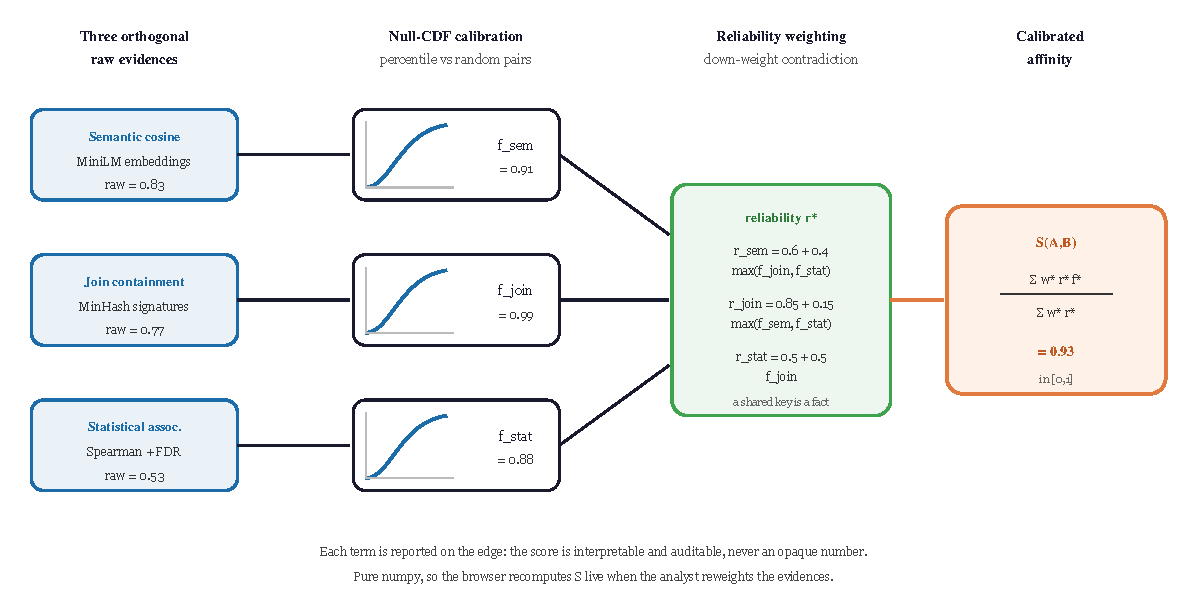
\includegraphics[width=0.98\textwidth]{fig-affinity.pdf}
\caption{The calibrated multi-evidence affinity. Three orthogonal raw evidences (semantic embedding cosine,
MinHash join containment, statistical association) are each mapped through their \emph{empirical null CDF}, i.e.
the percentile of the raw signal against a background sample of random dataset pairs, so a value near $1$ means
``far stronger than a random pair'' regardless of the raw scale. Reliability weights then discount an evidence
that contradicts the others (a high semantic match with no joinability is a weak reason to link; a shared key is
intrinsically reliable), and the fused score is the reliability-weighted, null-calibrated mean, reported
term-by-term. The whole computation is pure \texttt{numpy}, so an analyst can reweight the evidences and see the
graph re-rank live in the browser.}
\label{fig:affinity}
\end{figure*}

The core contribution is a single relatedness score that fuses the three orthogonal evidences of
Section~\ref{sec:evidence} (we fuse semantic, joinability, and statistical; the two remaining edge kinds are
provenance and geographic preconditions, not relatedness signals). Let a dataset pair $(A,B)$ have raw semantic
cosine $s$, raw join containment $j$, and raw statistical strength $t$. Two problems must be solved before these
can be added: their scales are not comparable (a cosine of $0.6$ and a containment of $0.6$ do not mean the same
thing), and a large raw value is not the same as a \emph{surprising} one.

\textbf{Null calibration.} We solve both by mapping each raw signal through its \emph{empirical null cumulative
distribution}. For evidence $e\in\{s,j,t\}$ we draw a background sample of the raw signal over random dataset
pairs and fit its empirical CDF $\widehat{F}_e$; the calibrated evidence is its percentile,
\begin{equation}
f_e \;=\; \widehat{F}_e(e) \;=\; \Pr\big[\,E_e \le e \,\big|\, \text{random pair}\,\big] \;\in\; [0,1],
\end{equation}
computed by a binary search in the sorted background sample. After calibration, $f_e$ is directly interpretable
as ``this pair's evidence $e$ is stronger than a fraction $f_e$ of random pairs'', on a common $[0,1]$ scale for
all three evidences. The background samples (small sorted arrays) are fit offline and shipped with the graph so
the calibration is reproducible and available in the browser.

\textbf{Reliability weighting.} Orthogonal evidences should not be trusted equally when they disagree. A high
semantic similarity with no joinability is often topical coincidence (two datasets both mention ``education''),
whereas a strong shared key with no semantic echo is still a real structural link. We encode this with gentle
reliability multipliers in $[0.5,1]$ that raise an evidence when the others agree and lower it when they do not:
\begin{align}
r_s &= 0.6 + 0.4\,\max(f_j, f_t), \\
r_j &= 0.85 + 0.15\,\max(f_s, f_t), \\
r_t &= 0.5 + 0.5\,f_j .
\end{align}
Joinability starts high (a shared key is a fact, lightly boosted by agreement); statistical association is trusted
only in proportion to a joinable alignment (without a real alignment the correlation is dubious); the semantic
term is fully trusted only with some structural or statistical support.

\textbf{Fusion.} With base evidence weights $w_s,w_j,w_t$ (default $0.34,0.40,0.26$; user-adjustable), the fused
affinity is the reliability-weighted, null-calibrated convex combination
\begin{equation}
S(A,B) \;=\; \frac{w_s r_s f_s + w_j r_j f_j + w_t r_t f_t}{w_s r_s + w_j r_j + w_t r_t}\;\in\;[0,1],
\end{equation}
with $S=0$ when the denominator vanishes. The result is monotone in each calibrated evidence, invariant to the
overall scale of the weights (the denominator renormalises), and, crucially, \emph{reported term by term}: every
affinity edge stores $f_s,f_j,f_t$ and the effective weights $w_e r_e$, so a reader can see \emph{why} two
datasets are linked and never confronts an opaque number. Figure~\ref{fig:affinity} shows the pipeline on a
worked pair. Because the whole computation is a handful of \texttt{numpy} operations over small per-pair vectors
and shipped background arrays, the browser recomputes $S$ for the visible subgraph in real time as the analyst
moves the evidence weights, which turns the score from a fixed ranking into an interactive instrument for asking
``rank these datasets as if I cared mostly about joinability'' versus ``\dots mostly about statistical echo''.

\section{Adversarial Validation}\label{sec:validation}

\begin{figure}[!t]
\centering
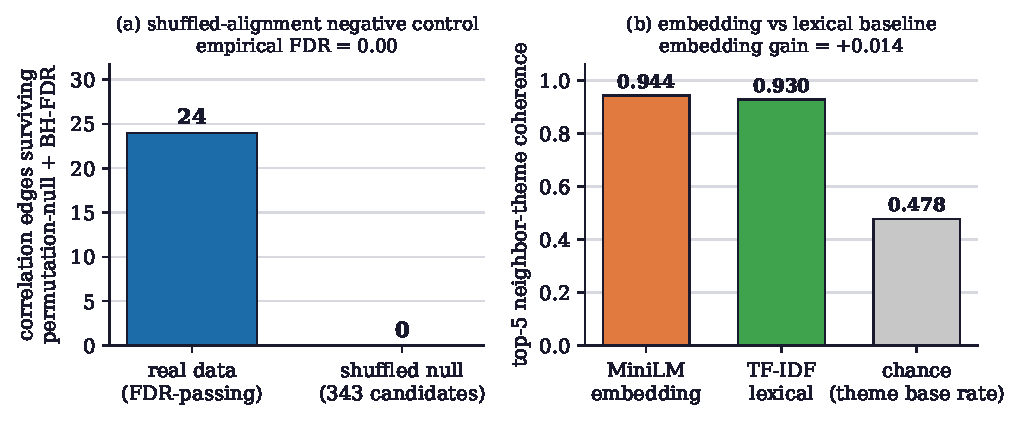
\includegraphics[width=0.99\columnwidth]{fig-validation.pdf}
\caption{Adversarial validation, from the committed metrics. \textbf{(a)} The empirical false-discovery gate:
the correlation miner accepts $24$ edges on the real data, but re-running the \emph{identical} test family on
\emph{shuffled} key alignments (breaking any true association) leaves $0$ survivors out of $343$ candidates, an
empirical false-discovery rate of $0.00$. \textbf{(b)} Honest SOTA-versus-classical: the MiniLM embedding reaches
$0.944$ top-$5$ neighbour-theme coherence against $0.930$ for a TF--IDF lexical baseline over the same text, both
far above the theme base rate of $0.478$; the true embedding gain is a modest $+0.014$, reported rather than
overstated.}
\label{fig:validation}
\end{figure}

The honest question about a relatedness graph is not ``did we find links'' but ``are the links stronger than a
null world''. We answer it with four adversarial or leakage-safe checks, all computed in the evaluation stage and
committed to \texttt{metrics.json}.

\textbf{The empirical false-discovery gate (the key check).} The correlation edges are the ones most easily
faked by multiple testing, so we subject them to a negative control. We take the exact indicator series and key
alignments used to mine correlations, \emph{shuffle} the key labels of each series to destroy any true
alignment, and re-run the identical pipeline: Spearman, seeded permutation null, Benjamini--Hochberg control at
$q=0.05$. A trustworthy miner should find essentially nothing on shuffled data. It finds nothing: of $343$
candidate pairs that clear the effect-size screen on the shuffled data, \textbf{$0$} survive the null and FDR
control, an empirical false-discovery rate of \textbf{$0.00$} (Fig.~\ref{fig:validation}a). This is the empirical
warrant for believing the $24$ correlations reported on real data; without it, ``survived FDR'' is a promise, not
a measurement.

\textbf{Honest SOTA-versus-classical.} It is tempting to justify a learned embedding by asserting it beats a
lexical baseline; we measure the gap instead. Over the identical set of datasets we compute top-$5$
neighbour-theme coherence (the fraction of a dataset's five nearest neighbours sharing its theme, a
leakage-free proxy for embedding quality) twice: once from MiniLM cosine, once from a TF--IDF lexical
similarity~\cite{tfidf} over the same text. The embedding reaches $0.944$ and the lexical baseline $0.930$, both
far above the theme base rate of $0.478$ (Fig.~\ref{fig:validation}b). The SOTA gain is a real but modest
$+0.014$; reporting it honestly is the point, and it justifies using the embedding as \emph{one} calibrated
evidence rather than as the whole ranking.

\textbf{Joinability sanity and semantic coherence.} Two further checks bound the graph's internal consistency.
Every \textbf{JOINABLE\_ON} edge should connect datasets that share a declared entity key; the measured fraction
is $1.000$ over all $117$ join edges (a drop would signal a bug). And the semantic neighbourhood is coherent:
across $4{,}753$ scored top-$k$ neighbour slots, $0.940$ share the source dataset's theme, far above the base
rate. Together with an isolated-node fraction of $0.0049$ (almost every dataset participates in at least one
relation), these establish that the graph is connected, internally consistent, and not an artifact of a leaky
test.

\section{Results: The Relatedness Graph}\label{sec:results}

\begin{figure}[!t]
\centering
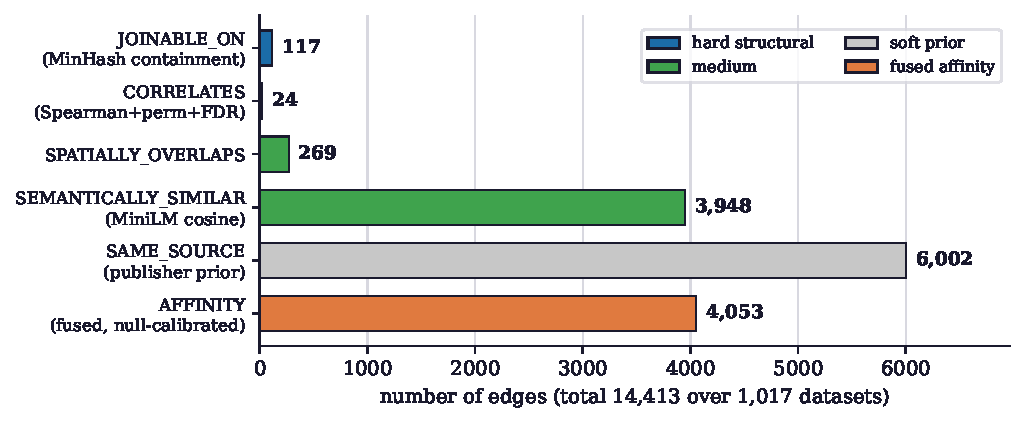
\includegraphics[width=0.99\columnwidth]{fig-evidence.pdf}
\caption{Edge-kind composition of the committed graph ($14{,}413$ edges over $1{,}017$ datasets), coloured by
evidence strength. The graph is honest about its own evidence hierarchy: a small number of \emph{hard} structural
links ($117$ joins, $24$ FDR-passing correlations), more \emph{medium} semantic and spatial evidence, a large but
\emph{soft} same-source prior, and the $4{,}053$ fused, null-calibrated affinity summaries. The interface renders
the same hierarchy so an analyst is never invited to read a cheap prior as a strong relation.}
\label{fig:evidence}
\end{figure}

The committed graph over the $1{,}017$-dataset catalog has $14{,}413$ edges (Fig.~\ref{fig:evidence}):
$6{,}002$ SAME\_SOURCE, $3{,}948$ SEMANTICALLY\_SIMILAR, $269$ SPATIALLY\_OVERLAPS, $117$ JOINABLE\_ON, $24$
CORRELATES, and $4{,}053$ AFFINITY summary edges. The composition itself is part of the honesty: the vast
majority of raw edges are cheap priors and topical similarities, while the structurally hard evidence (joins and
FDR-passing correlations) is a small, carefully gated minority. The affinity score exists precisely so that this
mixture can be collapsed into one calibrated number per pair without losing the distinction, since a pair with a
strong join and a statistical echo scores far above a pair that is merely same-source.

Three concrete edges illustrate what the graph surfaces. The highest-affinity pair,
\dsname{Nombramientos Sistema de Alta Direcci\'on P\'ublica} and \dsname{Convocatorias Sistema de Alta
Direcci\'on P\'ublica} (appointments and calls of the senior public-management system), scores $S=0.999$ with
$f_s=0.999$, $f_j=1.000$, $f_t=0.999$: two tables of the same administrative process, near-identical in text,
perfectly joinable, and statistically aligned, exactly the pair a human would call ``obviously the same family''.
A representative correlation edge links \dsname{Establecimientos educacionales} and \dsname{Establecimientos de
salud vigentes} (educational and active health establishments) at $\rho=0.528$, adjusted $p=0.001$, over $n=324$
municipalities aligned on \dsname{comuna\_cut}: schools and health facilities co-locate across municipalities, a
relation that survives the permutation null, FDR control, and the partial-correlation guard, and which we report
as an association, not a cause. A representative join edge connects two municipality-keyed tables with MinHash
containment $0.769$ on their \dsname{comuna} columns, recording the exact columns and set sizes so the join is
executable, not merely suggested. Each of these is inspectable in the live instance with its full evidence.

\section{Honest Scope and Limitations}\label{sec:scope}

The graph reports \emph{potential} relatedness with calibrated, auditable strength; it does not assert causation
and it is tuned for one catalog. Five limitations are worth stating plainly.

\textbf{Association, not causation.} A CORRELATES edge means two indicators move together across municipalities
after a permutation null, FDR control, and a first-order partial-correlation guard against a single common
driver. It does not identify a mechanism, and a higher-order confounder can still induce it. The interface labels
these edges as associations.

\textbf{Evidence hierarchy is real and unequal.} Of the $14{,}413$ edges, only $117+24$ are structurally hard;
the rest are priors or topical similarities. The affinity weighting encodes this, but a user who reweights all
mass onto the semantic evidence will get a graph dominated by topical coincidence. The reliability multipliers
mitigate but do not eliminate this, and the interface keeps the raw evidence visible for exactly this reason.

\textbf{Catalog-specific tuning.} The alignment keys (\dsname{comuna\_cut}, region), the government-Chile entity
vocabulary, and the thresholds (semantic $\ge 0.45$, containment $\ge 0.5$, $|\rho|\ge 0.35$, minimum overlap
$8$, $q=0.05$) are set for this catalog. The \emph{method} transfers, but the exact tunables would need
re-fitting for another portal, and the null backgrounds would need re-sampling.

\textbf{Deliberately light statistics.} The correlation miner uses Spearman with a permutation null rather than a
heavier dependence measure, and the affinity uses first-order (not full) reliability interactions. This is a
conscious trade for a stack that runs identically offline and in the browser; a server-side variant could use
richer dependence estimators at the cost of the live lane.

\textbf{Coverage.} Full table profiling covers the $303$-dataset government direct-file tier; datasets outside it
are catalogued and embedded from metadata but do not contribute join or correlation evidence, so their edges rest
on the semantic and same-source signals only. The graph is honest about this: such datasets simply carry no hard
structural edges.

\section{Reproducibility and Availability}\label{sec:repro}

Every number in this paper comes from artifacts committed to the repository: the graph
(\texttt{graph.json}), the evaluation metrics (\texttt{metrics.json}), the harvest report
(\texttt{harvest\_report.json}), and the per-case artifacts. The three figures are regenerated deterministically
by a single script from those artifacts (the two data figures) and from a hand-authored, theme-aware vector
schematic (the method figure), with no network access. The pipeline is staged, seeded, and gated by
determinism and data-contract tests. The relatedness statistics and the affinity are pure \texttt{numpy}/%
\texttt{math}, so the same code runs in the offline pipeline and in the browser live lane; the graph is also
queryable from an agent via an included MCP server. Source, artifacts, and a live instance are open under the MIT
license at \url{https://github.com/fsantibanezleal/CAOS_ATALAYA} and \url{https://atalaya.fasl-work.com}.

\section{Conclusion}

Atalaya turns a flat national open-data catalog into an auditable relatedness graph by fusing three orthogonal
evidences into a single calibrated score, and by holding that graph to an adversarial standard rather than a
plausibility standard. The calibration against empirical null distributions makes a score mean ``stronger than
chance''; the reliability weighting makes contradicting evidence count for less; the term-by-term reporting makes
every edge auditable; and the empirical false-discovery gate ($0$ of $343$ shuffled correlations survive) makes
the statistical edges believable in a way an uncontrolled miner cannot claim. The honest SOTA-versus-classical
margin ($+0.014$) is reported rather than oversold, in keeping with the system's premise that a data map is only
useful if it can be trusted. The method is not tied to this catalog; what transfers is the recipe of fuse,
calibrate against a null, weight by reliability, and gate against a shuffled negative control, for anyone building
a relatedness graph over a large, heterogeneous collection of datasets.

\appendices

\section{Configuration and Null Construction}\label{app:config}

For exact reproduction, the relation-mining tunables are: semantic top-$k=8$ with minimum cosine $0.45$; join
minimum MinHash containment $0.50$ on the anchor keys \dsname{comuna\_cut} and region; correlation minimum shared
key values $8$, minimum $|\rho|\;0.35$, at most $6$ indicator columns per dataset, a global cap of $40{,}000$
correlation tests (logged if reached), and Benjamini--Hochberg control at $q=0.05$. The permutation null uses a
seeded generator ($2{,}000$ permutations in the miner, $500$ in the negative control) with add-one smoothing so a
reported $p$-value is never exactly zero. The empirical null CDF for each affinity evidence is fit offline by
sampling the raw signal over random dataset pairs, sorting the sample, and evaluating the percentile by binary
search at query time; the sorted sample is shipped with the graph so the calibration is identical offline and in
the browser. Default affinity weights are $w_s=0.34$, $w_j=0.40$, $w_t=0.26$ and are renormalised by the fusion
denominator, so only their ratios matter.

\balance

\begin{thebibliography}{00}

\bibitem{fair} M.~D. Wilkinson \emph{et al.}, ``The FAIR guiding principles for scientific data management and
stewardship,'' \emph{Scientific Data}, vol.~3, art.~160018, 2016. doi:10.1038/sdata.2016.18.

\bibitem{aurum} R.~C. Fernandez \emph{et al.}, ``Aurum: A data discovery system,'' in \emph{Proc. IEEE 34th Int.
Conf. Data Engineering (ICDE)}, 2018, pp.~1001--1012. doi:10.1109/ICDE.2018.00094.

\bibitem{auctus} S.~Castelo \emph{et al.}, ``Auctus: A dataset search engine for data discovery and
augmentation,'' \emph{Proc. VLDB Endowment}, vol.~14, no.~12, pp.~2791--2794, 2021.
doi:10.14778/3476311.3476346.

\bibitem{minhash} A.~Z. Broder, ``On the resemblance and containment of documents,'' in \emph{Proc. Compression
and Complexity of Sequences (SEQUENCES)}, 1997, pp.~21--29. doi:10.1109/SEQUEN.1997.666900.

\bibitem{lazo} R.~C. Fernandez \emph{et al.}, ``Lazo: A cardinality-based method for coupled estimation of
Jaccard similarity and containment,'' in \emph{Proc. IEEE 35th Int. Conf. Data Engineering (ICDE)}, 2019,
pp.~1190--1201. doi:10.1109/ICDE.2019.00109.

\bibitem{lshensemble} E.~Zhu, F.~Nargesian, K.~Q. Pu, and R.~J. Miller, ``LSH Ensemble: Internet-scale domain
search,'' \emph{Proc. VLDB Endowment}, vol.~9, no.~12, pp.~1185--1196, 2016. doi:10.14778/2994509.2994534.

\bibitem{sbert} N.~Reimers and I.~Gurevych, ``Sentence-BERT: Sentence embeddings using Siamese BERT-networks,''
in \emph{Proc. Conf. Empirical Methods in Natural Language Processing (EMNLP-IJCNLP)}, 2019, pp.~3982--3992.
doi:10.18653/v1/D19-1410.

\bibitem{minilm} W.~Wang, F.~Wei, L.~Dong, H.~Bao, N.~Yang, and M.~Zhou, ``MiniLM: Deep self-attention
distillation for task-agnostic compression of pre-trained transformers,'' in \emph{Advances in Neural
Information Processing Systems (NeurIPS)}, 2020. arXiv:2002.10957.

\bibitem{gds} D.~Brickley, M.~Burgess, and N.~Noy, ``Google Dataset Search: Building a search engine for
datasets in an open web ecosystem,'' in \emph{Proc. World Wide Web Conf. (WWW)}, 2019, pp.~1365--1375.
doi:10.1145/3308558.3313685.

\bibitem{tfidf} K.~Sp\"arck Jones, ``A statistical interpretation of term specificity and its application in
retrieval,'' \emph{Journal of Documentation}, vol.~28, no.~1, pp.~11--21, 1972. doi:10.1108/eb026526.

\bibitem{profiling} Z.~Abedjan, L.~Golab, and F.~Naumann, ``Profiling relational data: A survey,'' \emph{The
VLDB Journal}, vol.~24, no.~4, pp.~557--581, 2015. doi:10.1007/s00778-015-0389-y.

\bibitem{spearman} C.~Spearman, ``The proof and measurement of association between two things,'' \emph{The
American Journal of Psychology}, vol.~15, no.~1, pp.~72--101, 1904. doi:10.2307/1412159.

\bibitem{bh} Y.~Benjamini and Y.~Hochberg, ``Controlling the false discovery rate: A practical and powerful
approach to multiple testing,'' \emph{Journal of the Royal Statistical Society: Series B}, vol.~57, no.~1,
pp.~289--300, 1995. doi:10.1111/j.2517-6161.1995.tb02031.x.

\bibitem{partialcorr} K.~Baba, R.~Shibata, and M.~Sibuya, ``Partial correlation and conditional correlation as
measures of conditional independence,'' \emph{Australian \& New Zealand Journal of Statistics}, vol.~46, no.~4,
pp.~657--664, 2004. doi:10.1111/j.1467-842X.2004.00360.x.

\bibitem{pca} I.~T. Jolliffe and J.~Cadima, ``Principal component analysis: A review and recent developments,''
\emph{Philosophical Transactions of the Royal Society A}, vol.~374, art.~20150202, 2016.
doi:10.1098/rsta.2015.0202.

\bibitem{rustworkx} M.~Treinish \emph{et al.}, ``rustworkx: A high-performance graph library for Python,''
\emph{Journal of Open Source Software}, vol.~7, no.~79, art.~3968, 2022. doi:10.21105/joss.03968.

\end{thebibliography}

\end{document}
